\documentclass[12pt,a4paper]{jarticle}
\usepackage[dvipdfmx]{graphicx}
\graphicspath{{../png/}}

\begin{document}
\section{塩分変化のコンター}
\begin{figure}[hbtp]
    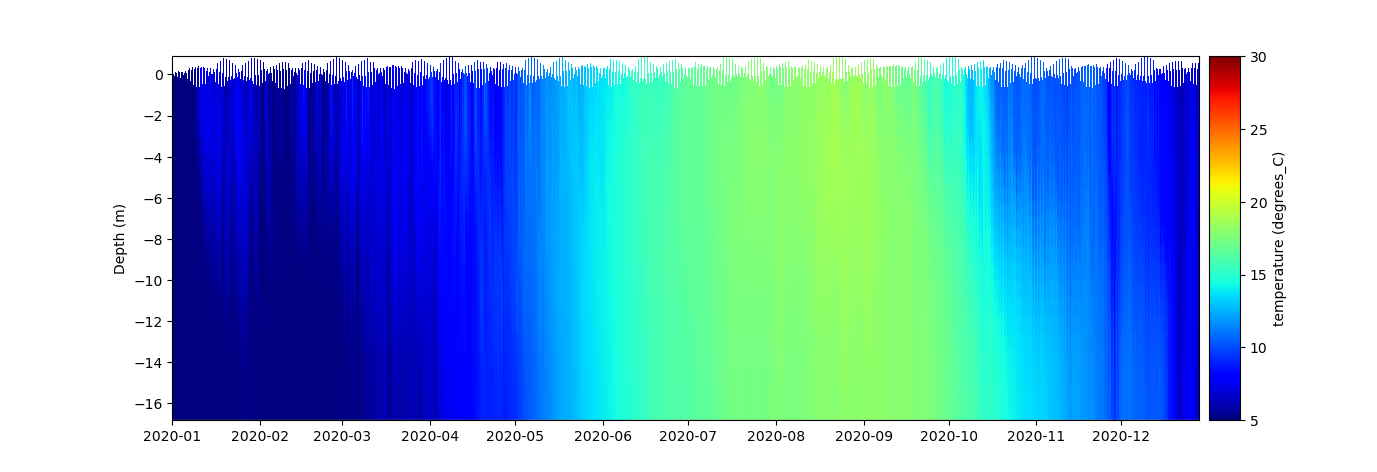
\includegraphics[keepaspectratio,width=180mm]{contour/Tokyo3_chiba1buoy.png}
    \caption{河川流量0.8倍}
\end{figure}

\begin{figure}[hbtp]
    \centering
        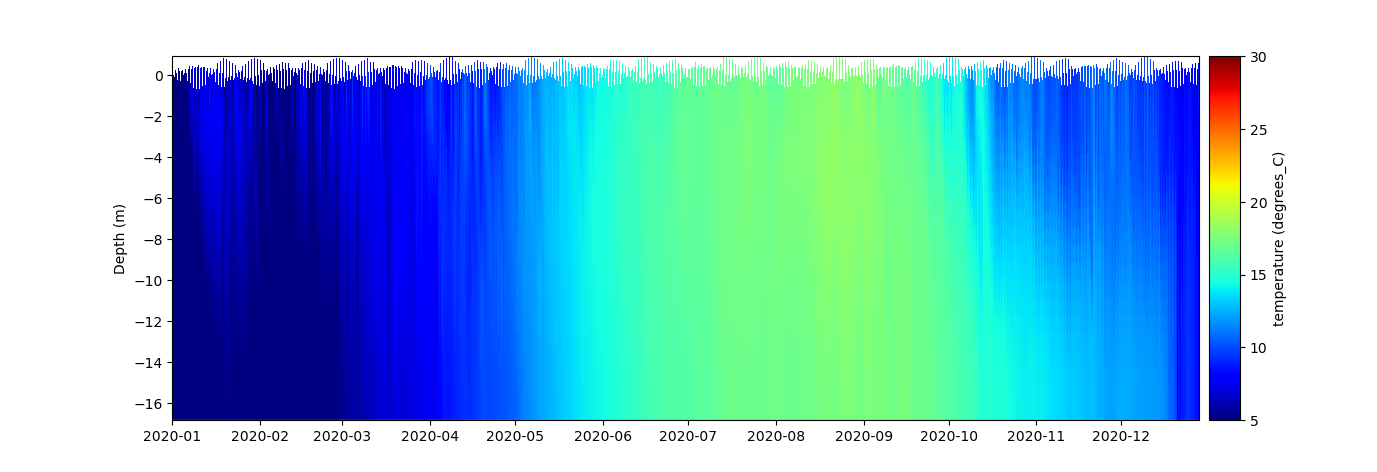
\includegraphics[keepaspectratio,scale=0.5]{contour/Tokyo4_chiba1buoy.png}
    \caption{河川流量1倍}
\end{figure}

\begin{figure}[hbtp]
    \centering
        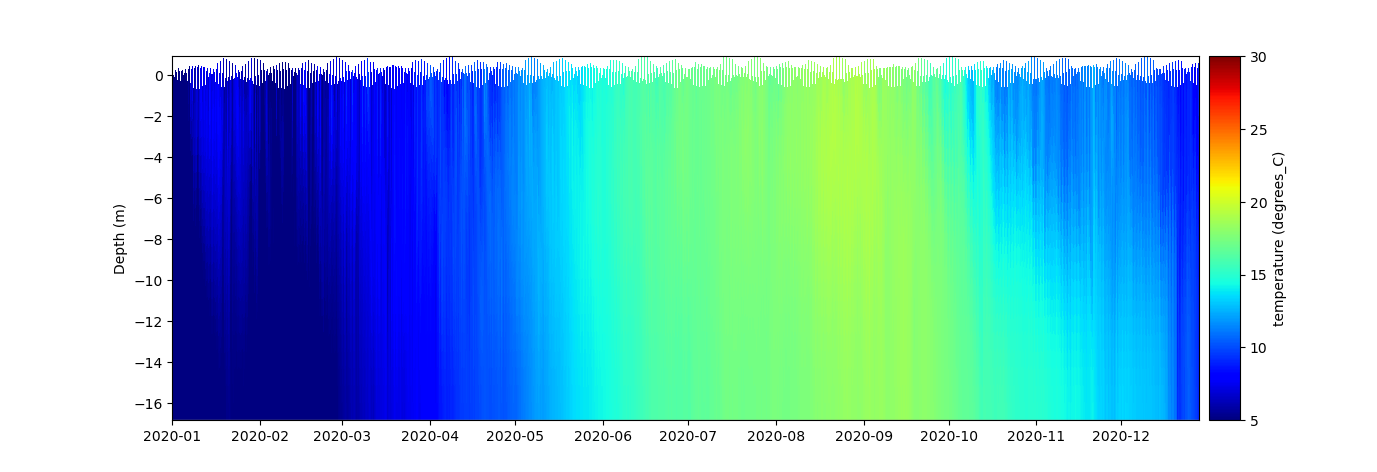
\includegraphics[keepaspectratio,scale=0.5]{contour/Tokyo5_chiba1buoy.png}
    \caption{河川流量1.2倍}
\end{figure}

\begin{figure}[hbtp]
    \centering
        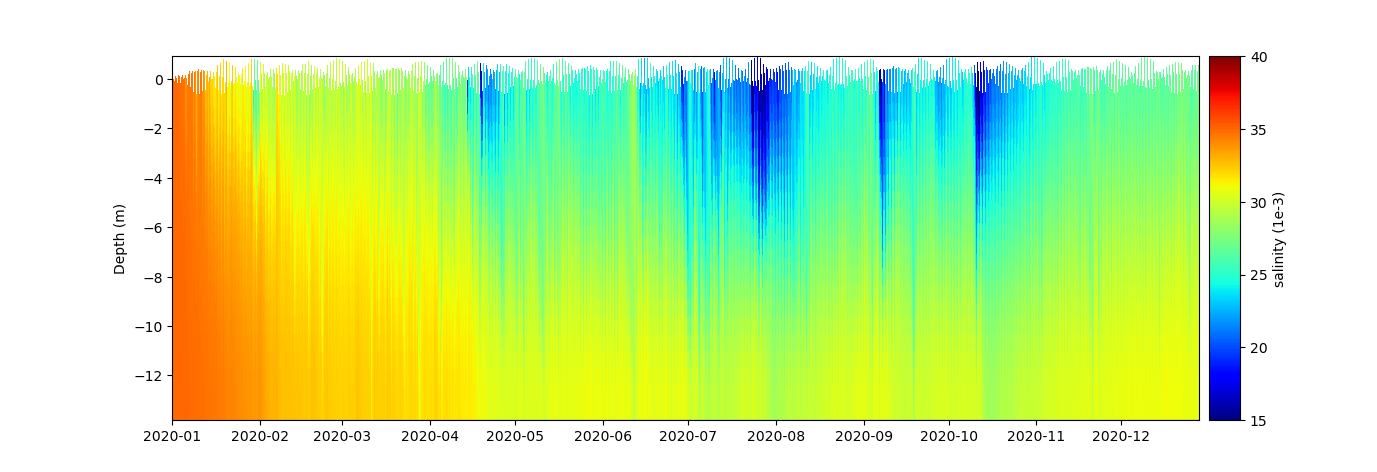
\includegraphics[keepaspectratio,scale=0.5]{contour/Tokyo6_chiba1buoy.png}
    \caption{河川流量1.5倍}
\end{figure}

\newpage
\section{河川流量等倍時のsigma layerごとでの塩分変化}
\begin{figure}[hbtp]
    \centering
        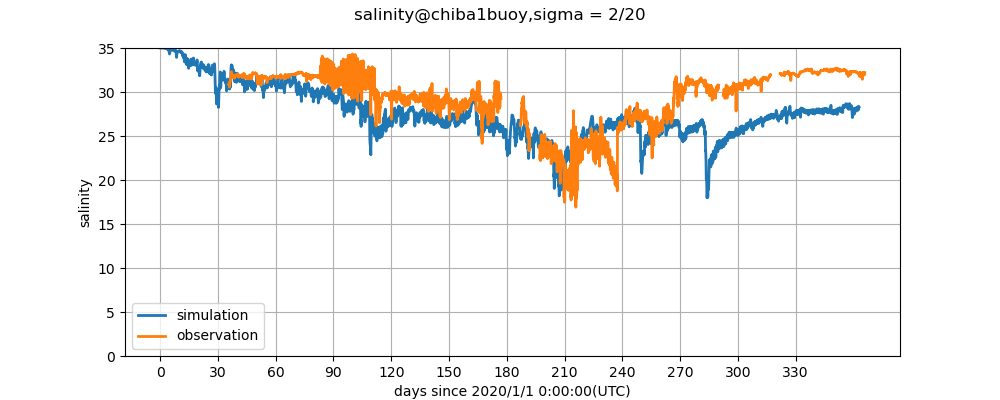
\includegraphics[keepaspectratio,scale=0.5]{Tokyo4/salinity_chiba1buoy_2_Tokyo4.png}
    \caption{siglay=2}
\end{figure}

\begin{figure}[hbtp]
    \centering
        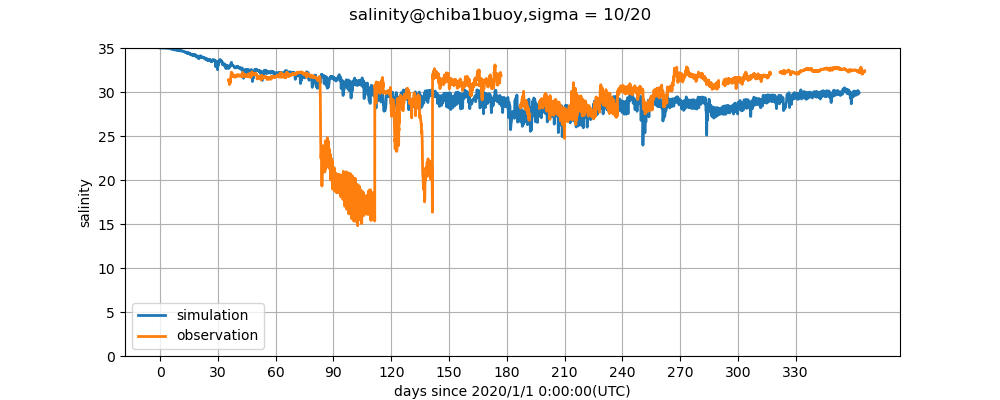
\includegraphics[keepaspectratio,scale=0.5]{Tokyo4/salinity_chiba1buoy_10_Tokyo4.png}
    \caption{siglay=10}
\end{figure}

\begin{figure}[hbtp]
    \centering
        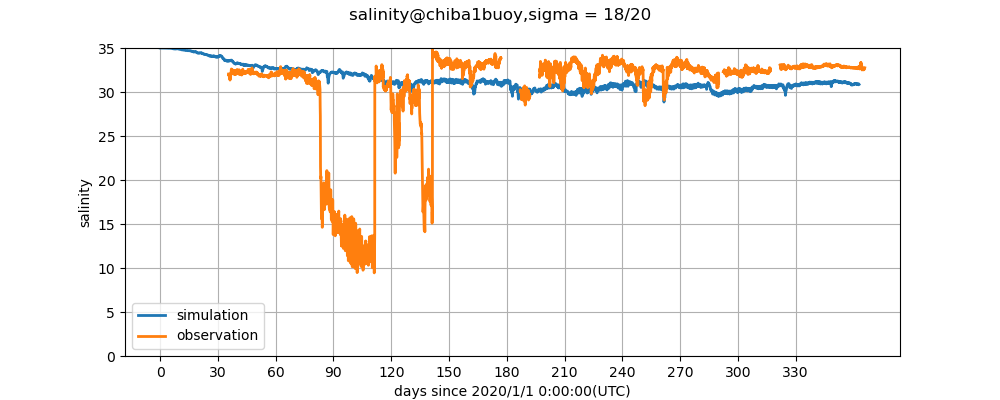
\includegraphics[keepaspectratio,scale=0.5]{Tokyo4/salinity_chiba1buoy_18_Tokyo4.png}
    \caption{siglay=18}
\end{figure}

\newpage
\section{河川流量1.5倍時のsigma layerごとでの水温変化}
\begin{figure}[hbtp]
    \begin{tabular}{cc}
      \begin{minipage}[t]{0.45\hsize}
        \centering
        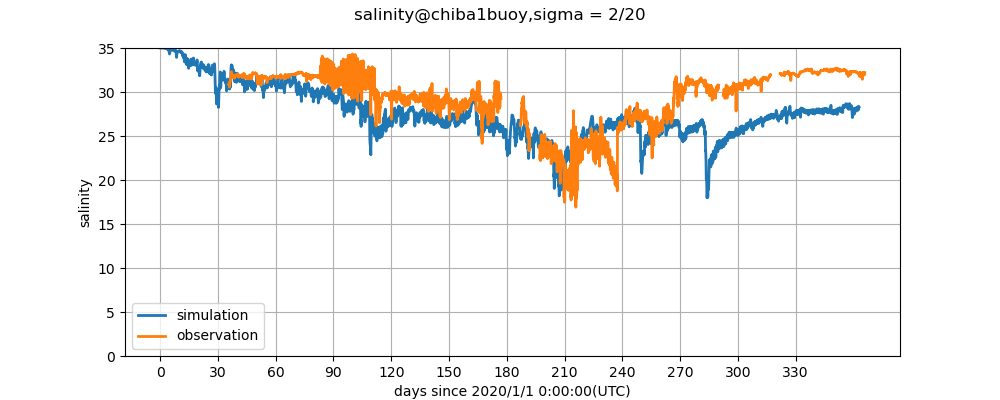
\includegraphics[keepaspectratio, scale=0.45]{Tokyo4/salinity_chiba1buoy_2_Tokyo4.png}
        \caption{siglay=2}
      \end{minipage} &
      \begin{minipage}[t]{0.45\hsize}
        \centering
        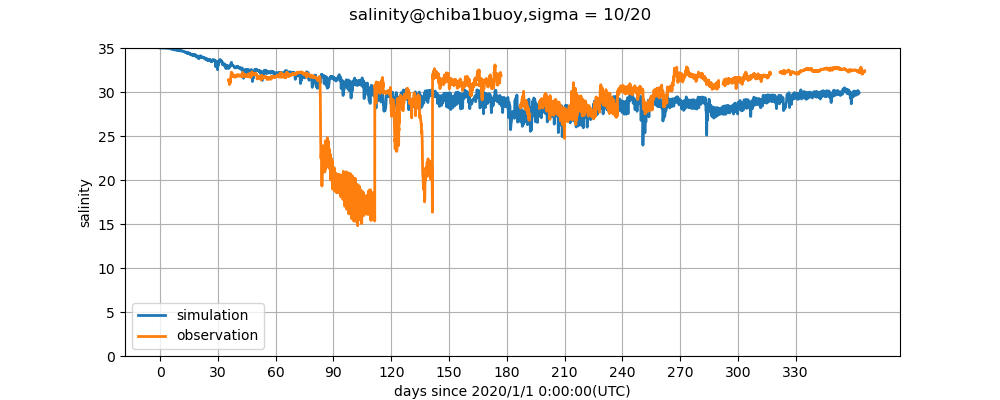
\includegraphics[keepaspectratio, scale=0.45]{Tokyo4/salinity_chiba1buoy_10_Tokyo4.png}
        \caption{siglalay=10}
      \end{minipage} 
      \begin{minipage}[t]{0.45\hsize}
        \centering
        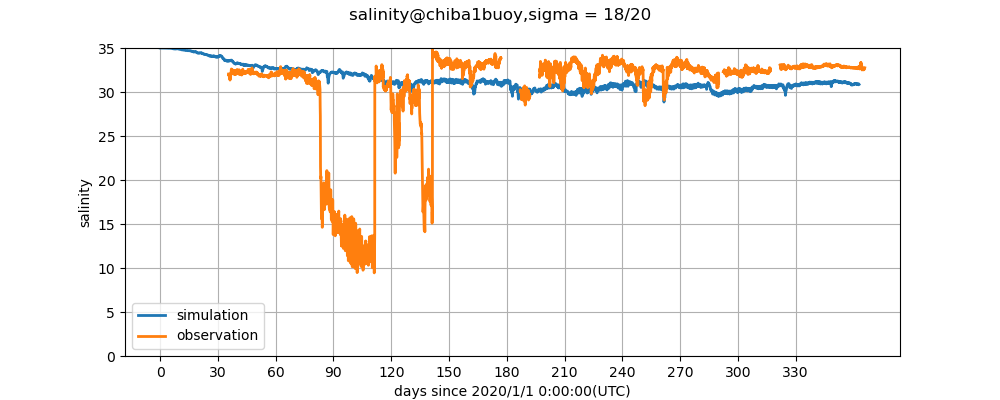
\includegraphics[keepaspectratio, scale=0.45]{Tokyo4/salinity_chiba1buoy_18_Tokyo4.png}
        \caption{siglay=18}
      \end{minipage}
    \end{tabular}
  \end{figure}




        
\end{document}

